\chapter{Massa ed energia di legame}

Nel capitolo precedente abbiamo studiato \emph{come} avvengono i decadimenti, ma non abbiamo mai risposto alla domanda di fondo: perché alcuni nuclei sono più stabili di altri? Che cosa governa la topologia della carta dei nuclidi? 

La risposta sta nell'energia di legame, legata all'energia potenziale della forza nucleare. Prima però bisogna saper misurare la massa di un nucleo. 

\section{Sistemi legati}

Se consideriamo un nucleo come un insieme di $Z$ protoni e $N$ neutroni, verrebbe naturale scrivere $M_{\text{nucleo}} = Z m_p + N m_n$, con $A = N + Z$. Questo però non è corretto, perché il nucleo è un \emph{sistema legato}\mkeyword{sistema legato}, cioè un insieme di corpi caratterizzato da energia meccanica totale negativa.\footnote{Cosa che comporta un confinamento, in quanto $U(r) = E - T \leq E$, ma sappiamo che per $r \to \infty$ si ha $U \to 0$ ma dato che $E < 0$, per definizione di sistema legato, deve esistere $r_{max}$ tale per cui $U(r_{max}) = E$ e quindi si deve avere $r \leq r_{max}$} \\
Quando i nucleoni si legano, infatti, emettono energia verso l'esterno: nel caso atomico un fotone, nel caso nucleare, un $\gamma$ o energia cinentica dei prodotti. 

Per un sistema legato vale allora
%
\begin{tcolorbox}[colback=yellow!10!white, colframe=orange!70!black, boxrule=0.8pt]
\begin{equation}
    M_{\text{sistema legato}} = \sum_i M_i - B \qquad \Longrightarrow \qquad B = \sum_i M_i - M_{\text{sistema legato}} = \Delta M
    \label{eq:def_B}
\end{equation}
\end{tcolorbox}
dove $B > 0$ è l'energia di legame\mkeyword{energia di legame}, cioè l'energia necessaria per separare il sistema nei suoi costituenti. \\
L'energia da fornire al sistema è esattamente $B$ perché separare il sistema significa riportarlo nella configurazione di partenza quando protoni e neutroni non erano legati e il bilancio energetico tra le due configurazioni è $B$. \\
Sistemi con energia di legame più alta necessitano di maggiore energia per essere separati.

È interessante stimare l'ordine di grandezza di $\Delta M/M$, perché permette di confrontare tra loro sistemi legati di natura completamente diversa. \\

Consideriamo il caso a $2$ corpi: la variazione di massa è pari all'energia meccanica totale
%
\begin{equation}
    \Delta M = T + U \qquad \text{con} \qquad T = \frac{1}{2} \mu v^2
\end{equation}
e, imponendo che la forza fornisca l'accelerazione centripeta su un'orbita di raggio $R$,
%
\begin{equation}
    \frac{dU}{dr} = \frac{\mu v^2}{R} \qquad \Longrightarrow \qquad \Delta M = U + \frac{1}{2} R \frac{dU}{dr}
\end{equation}
da cui, dividendo per la massa del sistema,
%
\begin{equation}
    \frac{\Delta M}{M} = \frac{U + \frac{1}{2} R \frac{dU}{dr}}{M c^2}
\end{equation}
Consideriamo adesso un'energia potenziale del tipo $U = - g^2/r$, per cui $dU/dr = + g^2/r^2$, e valutiamo in $r = R$
%
\begin{equation}
    \frac{\Delta M}{M} = \frac{- \dfrac{g^2}{R} + \dfrac{1}{2} \dfrac{g^2}{R}}{M c^2} = - \frac{g^2}{2 M c^2 R}
\end{equation}
Moltiplicando e dividendo per $\hbar$ si ottiene una forma particolarmente espressiva
%
\begin{tcolorbox}[colback=yellow!10!white, colframe=orange!70!black, boxrule=0.8pt]
\begin{equation}
    \frac{\Delta M}{M} = - \frac{1}{2} \frac{g^2}{\hbar c} \cdot \frac{\hbar / M c}{R} = - \frac{1}{2} \alpha_g \frac{\lambda_C}{R}
\end{equation}
\end{tcolorbox}
dove $\alpha_g = g^2/\hbar c$ è una costante di accoppiamento adimensionale, $\lambda_C = \hbar/Mc$ è la lunghezza Compton del sistema e $R$ è la sua scala caratteristica. 

Il vantaggio di lavorare con quantità adimensionali è che la stessa formula si applica a un'ampia gamma di sistemi legati, come mostra la tabella seguente. 

\begin{table}[htbp]
\centering
\begin{tabular}{lc}
\hline
Sistema & $\Delta M / M$ \\
\hline
Terra--Sole & $\sim 10^{-9}$ \\
Cristallo & $\sim 10^{-10}$ \\
Atomo di idrogeno & $\sim 10^{-8}$ \\
Nucleo & $\sim 10^{-2}$ \\
\hline
\end{tabular}
\caption{Ordini di grandezza del difetto di massa relativo in alcuni sistemi legati.}
\label{tab:difetto_massa}
\end{table}

Il nucleo si distingue di molti ordini di grandezza da tutti gli altri: è questo il motivo per cui i fenomeni di fissione e fusione sono rilevanti per la produzione di energia, mentre nessuna reazione chimica può esserlo. 

\subsection{Dipendenza di \texorpdfstring{$B$}{B} da \texorpdfstring{$A$}{A}}

L'energia di legame cresce con il numero di nucleoni, perché più nucleoni ci sono più legami si formano. Per confrontare tra loro nuclei diversi conviene quindi studiare l'energia di legame \emph{per nucleone}
%
\begin{equation}
    \frac{B(A,Z)}{A}
\end{equation}
che rappresenta l'energia media necessaria per estrarre un singolo nucleone dal nucleo: tanto più questo valore è alto, tanto più il nucleo è stabile.\\

L'andamento di questa quantità, riportato in Fig. \ref{fig:binding_energy}, è ricavato da misure sperimentali. Dalla curva si leggono tre caratteristiche principali. 

Innanzitutto, per quasi tutti i nuclei si ha $B/A \approx 8$ MeV: la curva è notevolmente piatta su gran parte del suo dominio. È questo il fatto sperimentale più importante, perché implica che l'energia di legame sia approssimativamente proporzionale ad $A$ e non, come si potrebbe pensare, al numero di coppie di nucleoni. 

In secondo luogo la curva cresce rapidamente per $A$ piccolo, raggiunge un massimo di circa $8,8$ MeV nella regione $A \sim 56 \div 62$, e poi decresce lentamente. Il massimo corrisponde al cosiddetto ``gruppo del ferro'', che contiene quindi i nuclei più stabili in natura. 

Infine, nella regione dei nuclei leggeri la curva non è regolare ma presenta picchi pronunciati in corrispondenza di ${}^{4}\mathrm{He}$, ${}^{12}\mathrm{C}$ e ${}^{16}\mathrm{O}$, cioè di nuclei con $A$ multiplo di $4$ e con $N = Z$ pari. Questi nuclei sono anomalmente più legati dei loro vicini, cosa non spiegabile con un modello classico: si tratta di un effetto quantistico legato all'accoppiamento dei nucleoni, di cui terremo conto più avanti con il termine di pairing. 

\begin{figure}[htbp]
\centering
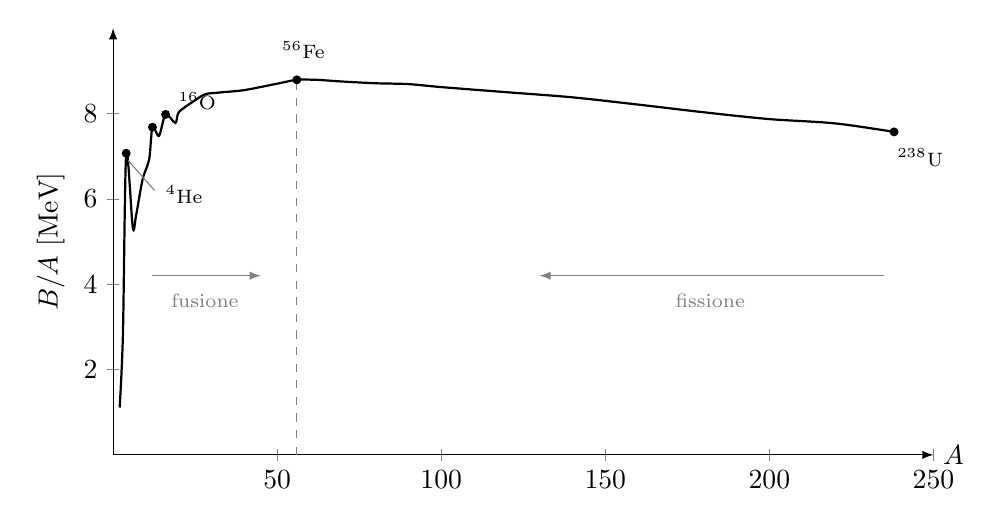
\begin{tikzpicture}
\begin{axis}[
    width=12cm, height=7cm,
    axis lines=left, axis line style={-latex},
    xlabel={$A$}, ylabel={$B/A$ [MeV]},
    xlabel style={at={(ticklabel* cs:1)}, anchor=west},
    xmin=0, xmax=250, ymin=0, ymax=10,
    xtick={50,100,150,200,250}, ytick={2,4,6,8},
    clip=false,
]
\addplot[black, thick, smooth] coordinates {
 (2,1.11) (3,2.83) (4,7.07) (6,5.33) (7,5.61) (9,6.46) (11,6.93) (12,7.68)
 (14,7.48) (16,7.98) (19,7.78) (20,8.03) (24,8.26) (28,8.45) (32,8.49)
 (40,8.55) (50,8.70) (56,8.79) (62,8.79) (70,8.75) (80,8.71) (90,8.69)
 (100,8.62) (120,8.50) (140,8.38) (160,8.21) (180,8.03) (200,7.87)
 (220,7.77) (238,7.57)
};
\addplot[only marks, mark=*, mark size=1.4pt] coordinates {(4,7.07) (12,7.68) (16,7.98) (56,8.79) (238,7.57)};
\node[anchor=west, font=\scriptsize] at (axis cs:13,6.1) {${}^{4}$He};
\draw[thin, gray] (axis cs:12.6,6.2) -- (axis cs:4.6,6.9);
\node[anchor=west, font=\scriptsize] at (axis cs:17,8.3) {${}^{16}$O};
\node[anchor=south, font=\scriptsize] at (axis cs:58,9.05) {${}^{56}$Fe};
\node[anchor=north west, font=\scriptsize] at (axis cs:236,7.4) {${}^{238}$U};
\draw[-latex, gray] (axis cs:12,4.2) -- (axis cs:45,4.2);
\node[anchor=north, font=\scriptsize, gray] at (axis cs:28,4.0) {fusione};
\draw[-latex, gray] (axis cs:235,4.2) -- (axis cs:130,4.2);
\node[anchor=north, font=\scriptsize, gray] at (axis cs:182,4.0) {fissione};
\draw[dashed, gray] (axis cs:56,0) -- (axis cs:56,8.79);
\end{axis}
\end{tikzpicture}
\caption{Energia di legame per nucleone in funzione del numero di massa.}
\label{fig:binding_energy}
\end{figure}

La forma della curva ha una conseguenza immediata. In natura si cerca sempre di massimizzare l'energia di legame per nucleone, favorendo i processi che portano verso nuclei più stabili: tutto il grafico può quindi essere letto come una discesa verso il picco del ferro da entrambi i lati. Si aprono allora due possibilità per guadagnare energia:
\begin{itemize}
    \item \emph{fondere} due nuclei leggeri per ottenerne uno più pesante, risalendo il ramo sinistro della curva (fusione nucleare);
    \item \emph{scindere} un nucleo pesante in nuclei più leggeri, risalendo il ramo destro (fissione nucleare).
\end{itemize}
In entrambi i casi il guadagno si legge direttamente come differenza di quota sul grafico, moltiplicata per il numero di nucleoni coinvolti. Nella fissione dell'uranio, ad esempio, si passa da $B/A \simeq 7,6$ MeV a $B/A \simeq 8,5$ MeV per frammenti di massa media $A \sim 118$, con un guadagno di circa $0,9$ MeV per nucleone, cioè un'energia dell'ordine di $200$ MeV per singola fissione. 

Nessuna reazione chimica può competere: lì le energie in gioco sono dell'ordine dell'eV, cioè $10^{6}$ volte più piccole, coerentemente con i rapporti $\Delta M/M$ della tabella \ref{tab:difetto_massa}.

\section{Masse atomiche e nucleari}

La distinzione tra masse atomiche e nucleari è fondamentale e usare le une al posto delle altre porta in alcuni casi a risultati sbagliati.\\

Trascurando l'energia di legame degli elettroni, che è dell'ordine dell'eV e quindi piccolissima rispetto alle energie in gioco, la massa atomica si scrive come
%
\begin{tcolorbox}[colback=yellow!10!white, colframe=orange!70!black, boxrule=0.8pt]
\begin{equation}
    M_{\text{at}}(A,Z) = M_{\text{nuc}}(A,Z) + Z m_e - B_{el} \simeq M_{\text{nuc}}(A,Z) + Z m_e
    \label{eq:massa_atomica}
\end{equation}
\end{tcolorbox}

Si definisce unità di massa atomica\mkeyword{unità di massa atomica} la quantità
%
\begin{equation}
    1 \ u = \frac{1}{12} M_{\text{at}}({}^{12}\mathrm{C}) = 931,5 \ \mathrm{MeV}
\end{equation}

\subsection{Masse nel decadimento \texorpdfstring{$\alpha$}{alfa}}

Consideriamo il decadimento
%
\begin{equation*}
    {}^{A}_{Z}\mathrm{X} \longrightarrow {}^{A-4}_{Z-2}\mathrm{Y} + {}^{4}_{2}\mathrm{He}
\end{equation*}
e scriviamo il $Q$-valore con le masse nucleari, che sono quelle fisicamente coinvolte nel processo
%
\begin{equation}
    Q = M_{\text{nuc}}({}^{A}_{Z}\mathrm{X}) - M_{\text{nuc}}({}^{A-4}_{Z-2}\mathrm{Y}) - M_{\text{nuc}}({}^{4}_{2}\mathrm{He})
\end{equation}
Usando la \eqref{eq:massa_atomica} per esprimere ciascun termine si ottiene
%
\begin{equation}
\begin{aligned}
    Q & = \big[ M_{\text{at}}({}^{A}_{Z}\mathrm{X}) - Z m_e \big] - \big[ M_{\text{at}}({}^{A-4}_{Z-2}\mathrm{Y}) - (Z-2) m_e \big] - \big[ M_{\text{at}}({}^{4}_{2}\mathrm{He}) - 2 m_e \big] \\[4pt]
    & = M_{\text{at}}({}^{A}_{Z}\mathrm{X}) - M_{\text{at}}({}^{A-4}_{Z-2}\mathrm{Y}) - M_{\text{at}}({}^{4}_{2}\mathrm{He}) - \big[ Z - (Z-2) - 2 \big] m_e
\end{aligned}
\end{equation}
e l'ultima parentesi è nulla, per cui
%
\begin{tcolorbox}[colback=yellow!10!white, colframe=orange!70!black, boxrule=0.8pt]
\begin{equation}
    Q_{\alpha} = M_{\text{at}}({}^{A}_{Z}\mathrm{X}) - M_{\text{at}}({}^{A-4}_{Z-2}\mathrm{Y}) - M_{\text{at}}({}^{4}_{2}\mathrm{He})
\end{equation}
\end{tcolorbox}
Nel decadimento $\alpha$ è quindi indifferente usare masse atomiche o nucleari, perché il numero totale di elettroni si conserva e i termini $m_e$ si semplificano. 

\subsection{Masse nel decadimento \texorpdfstring{$\beta$}{beta}}

Nel decadimento $\beta$ la situazione è diversa: il numero di elettroni \emph{non} si conserva, e le tre modalità vanno trattate separatamente.\\

Per il decadimento $\beta^-$, cioè ${}^{A}_{Z}\mathrm{X} \to {}^{A}_{Z+1}\mathrm{Y} + e^- + \bar{\nu}_e$, si ha
%
\begin{equation*}
\begin{cases}
    M_{\text{nuc}}({}^{A}_{Z}\mathrm{X}) = M_{\text{at}}({}^{A}_{Z}\mathrm{X}) - Z m_e \\[4pt]
    M_{\text{nuc}}({}^{A}_{Z+1}\mathrm{Y}) = M_{\text{at}}({}^{A}_{Z+1}\mathrm{Y}) - (Z+1) m_e
\end{cases}
\end{equation*}
e, trascurando la massa del neutrino,
%
\begin{equation}
\begin{aligned}
    Q & = M_{\text{nuc}}({}^{A}_{Z}\mathrm{X}) - M_{\text{nuc}}({}^{A}_{Z+1}\mathrm{Y}) - m_e \\[4pt]
      & = M_{\text{at}}({}^{A}_{Z}\mathrm{X}) - Z m_e - M_{\text{at}}({}^{A}_{Z+1}\mathrm{Y}) + (Z+1) m_e - m_e
\end{aligned}
\end{equation}
da cui
%
\begin{tcolorbox}[colback=yellow!10!white, colframe=orange!70!black, boxrule=0.8pt]
\begin{equation}
    Q_{\beta^-} = M_{\text{at}}({}^{A}_{Z}\mathrm{X}) - M_{\text{at}}({}^{A}_{Z+1}\mathrm{Y}) 
\end{equation}
\end{tcolorbox}
Anche qui le masse elettroniche si semplificano, ma per una ragione diversa dal caso $\alpha$: l'elettrone emesso compensa l'elettrone in più dell'atomo figlio.\\

Per il decadimento $\beta^+$, cioè ${}^{A}_{Z}\mathrm{X} \to {}^{A}_{Z-1}\mathrm{Y} + e^+ + \nu_e$, l'atomo figlio ha un elettrone in \emph{meno}, quindi $M_{\text{nuc}}({}^{A}_{Z-1}\mathrm{Y}) = M_{\text{at}}({}^{A}_{Z-1}\mathrm{Y}) - (Z-1) m_e$ e si ottiene
%
\begin{equation}
    Q = M_{\text{at}}({}^{A}_{Z}\mathrm{X}) - Z m_e - M_{\text{at}}({}^{A}_{Z-1}\mathrm{Y}) + (Z-1) m_e - m_e
\end{equation}
cioè
%
\begin{tcolorbox}[colback=yellow!10!white, colframe=orange!70!black, boxrule=0.8pt]
\begin{equation}
    Q_{\beta^+} = M_{\text{at}}({}^{A}_{Z}\mathrm{X}) - M_{\text{at}}({}^{A}_{Z-1}\mathrm{Y}) - 2 m_e
\end{equation}
\end{tcolorbox}
Qui i termini elettronici \emph{non} si cancellano: resta un contributo $-2m_e$, che è l'errore che si commetterebbe usando ingenuamente le masse atomiche come nel caso $\alpha$.\\

Infine, per la cattura elettronica ${}^{A}_{Z}\mathrm{X} + e^- \to {}^{A}_{Z-1}\mathrm{Y} + \nu_e$ l'elettrone catturato compare nello stato \emph{iniziale}
%
\begin{equation}
    Q = M_{\text{nuc}}({}^{A}_{Z}\mathrm{X}) + m_e - M_{\text{nuc}}({}^{A}_{Z-1}\mathrm{Y})
\end{equation}
e ripetendo la sostituzione si trova
%
\begin{tcolorbox}[colback=yellow!10!white, colframe=orange!70!black, boxrule=0.8pt]
\begin{equation}
    Q_{\varepsilon} = M_{\text{at}}({}^{A}_{Z}\mathrm{X}) - M_{\text{at}}({}^{A}_{Z-1}\mathrm{Y})
\end{equation}
\end{tcolorbox}
dove si è trascurata la differenza tra le energie di legame elettroniche dei due atomi.

\subsection{Due esempi}

La curva dell'energia di legame, che studieremo tra poco, spiega da dove le stelle prendano la loro energia. Il bilancio della catena protone-protone è
%
\begin{equation*}
    4 p \longrightarrow {}^{4}_{2}\mathrm{He} + 2 e^+ + 2 \nu_e
\end{equation*}
e, usando $m_p = 1,007276 \ u$, $m_{{}^4\mathrm{He}} = 4,001506 \ u$ e $m_{e} = 0,000548 \ u$,
%
\begin{equation}
    Q = 4 m_p - m_{{}^4\mathrm{He}} - 2 m_e = 0,026502 \ u = 24,68 \ \mathrm{MeV}
\end{equation}
In realtà il valore riportato è $Q \simeq 26,7$ MeV, che si ottiene con le masse atomiche: la differenza corrisponde all'annichilazione dei due positroni con due elettroni del mezzo.\\

Un altro esempio è la fissione. Per una reazione del tipo
%
\begin{equation*}
    {}^{235}_{92}\mathrm{U} \longrightarrow {}^{93}_{37}\mathrm{Rb} + {}^{140}_{55}\mathrm{Cs} + 2n
\end{equation*}
si può stimare l'energia liberata osservando che l'energia di legame per nucleone passa da circa $7,6$ MeV a circa $8,5$ MeV, con un guadagno di circa $0,9$ MeV per nucleone. Si ottiene quindi un'energia dell'ordine di $200 \div 230$ MeV per singola fissione. 

\section{Il modello a goccia}

Vogliamo adesso costruire un modello che riproduca la curva appena vista. 

Supponiamo in prima battuta che \emph{tutti} i nucleoni interagiscano con tutti: il numero di coppie è allora
%
\begin{equation}
    N_{\text{coppie}} = \binom{A}{2} = \frac{1}{2} A (A-1)
\end{equation}
e, detta $\bar{U}$ l'energia media per coppia, si avrebbe
%
\begin{equation}
    B \sim \frac{1}{2} \bar{U} A (A-1) \qquad \Longrightarrow \qquad \frac{B}{A} \sim \frac{1}{2} \bar{U} (A-1)
\end{equation}
Questo risultato è in netto contrasto con il dato sperimentale, che mostra $B/A$ pressoché costante. 

L'ipotesi va quindi corretta: non si ha un'interazione totale, ma ciascun nucleone interagisce soltanto con una parte del nucleo, definita da un \emph{volume efficace} $V_{\text{eff}}$. Si ottiene allora
%
\begin{equation}
    B \sim \frac{1}{2} \bar{U} A (A-1) \frac{V_{\text{eff}}}{V} \qquad \Longrightarrow \qquad \frac{B}{A} \sim \frac{1}{2} (A-1) \bar{U} \frac{V_{\text{eff}}}{V} \sim \frac{A \bar{U} V_{\text{eff}}}{V}
\end{equation}
che è costante, come osservato, purché $A/V$ sia costante, cioè purché
%
\begin{tcolorbox}[colback=yellow!10!white, colframe=orange!70!black, boxrule=0.8pt]
\begin{equation}
    V \propto A
\end{equation}
\end{tcolorbox}

Dalla condizione $A/V = $ cost segue che la densità di nucleoni è la stessa per tutti i nuclei: un nucleo con il doppio dei nucleoni occupa esattamente il doppio del volume. Questa è la proprietà che caratterizza i liquidi incomprimibili, nei quali le molecole stanno a contatto a una distanza fissata dal potenziale, ed è il motivo per cui si modellizza il nucleo come una goccia: da qui il nome di modello a goccia\mkeyword{modello a goccia}. 

Le conseguenze sono due. 

La prima è che l'interazione nucleare è a corto raggio, per cui si considerano solo interazioni tra nucleoni vicini. 

La seconda è che, essendo $V \propto A$,
%
\begin{equation}
    V = \frac{4}{3} \pi R^3 \propto A \quad \Longrightarrow \quad R = r_0 A^{1/3} \quad \text{e} \quad S \propto A^{2/3}
\end{equation}
con $r_0 \approx 1,25$ fm, in accordo con quanto si misura negli esperimenti di scattering. 

Quanto ottenuto finora fornisce un solo termine, proporzionale al numero di nucleoni
%
\begin{equation}
    B \simeq a_V A
\end{equation}
che però, confrontato con la Fig. \ref{fig:binding_energy}, riproduce soltanto il fatto che la curva sia approssimativamente piatta: prevede $B/A$ rigorosamente costante, mentre i dati mostrano una crescita per $A$ piccolo e una decrescita per $A$ grande. 

Il motivo è che nel ricavarlo abbiamo fatto tre approssimazioni grossolane:
\begin{itemize}
    \item abbiamo supposto che \emph{tutti} i nucleoni abbiano lo stesso numero di vicini, il che non vale per quelli sulla superficie;
    \item abbiamo considerato la sola interazione forte, ignorando la repulsione coulombiana tra protoni;
    \item abbiamo trattato i nucleoni come particelle classiche, ignorando che sono fermioni.
\end{itemize}

Andiamo quindi a scomporre $B$ in una somma di termini, ciascuno dei quali corregge una di queste approssimazioni
%
\begin{equation}
    B = B_V + B_S + B_C + B_A + B_p
\end{equation}
dove $B_V$ è il termine di volume appena ricavato, $B_S$ tiene conto dei nucleoni di superficie, $B_C$ della repulsione coulombiana, mentre $B_A$ e $B_p$, detti termini di asimmetria e di pairing, tengono conto della natura fermionica dei nucleoni e non sono previsti dal modello a goccia. 

Per i primi tre termini useremo direttamente le relazioni geometriche appena ricavate: è da $V \propto A$, $S \propto A^{2/3}$ e $R \propto A^{1/3}$ che si deducono le potenze di $A$ con cui ciascuna correzione scala. 

Il risultato finale sarà una formula \emph{semiempirica}: la forma funzionale di ogni termine viene da un argomento fisico, mentre i coefficienti sono ricavati da un fit ai dati sperimentali. Non si tratta quindi di una derivazione da principi primi, ma della parametrizzazione più semplice che riproduca la curva misurata con pochi parametri.

\subsection{Termine di volume e di superficie}

Da quanto detto, il termine dominante è proporzionale al numero di nucleoni
%
\begin{equation}
    B_V = a_V A
\end{equation}
L'approssimazione del volume efficace va però corretta sulla superficie: i nucleoni che si trovano sul bordo hanno meno vicini e sono quindi legati meno. Introduciamo allora un termine di superficie, negativo e proporzionale a $A^{2/3}$
%
\begin{equation}
    B_S = - a_S A^{2/3}
\end{equation}

\subsection{Termine coulombiano}

I protoni si respingono, e questo riduce l'energia di legame. Il termine è proporzionale al quadrato della carica e inversamente proporzionale al raggio
%
\begin{equation}
    B_C = - a_C \frac{Z^2}{A^{1/3}}
\end{equation}
La costante si può stimare a partire dall'energia coulombiana di una sfera uniformemente carica di carica $Ze$ e raggio $R_A = r_0 A^{1/3}$
%
\begin{equation}
    \frac{3}{5} \frac{(Ze)^2}{4 \pi \epsilon_0 R_A} = \frac{3}{5} \frac{Z^2}{A^{1/3}} \frac{\alpha \hbar c}{r_0} \approx 0,69 \ \mathrm{MeV} \ \frac{Z^2}{A^{1/3}}
\end{equation}
in ottimo accordo con il valore sperimentale $a_C \approx 0,72$ MeV. 

\subsection{Termine di asimmetria}

I termini visti finora trattano i nucleoni come particelle classiche. In realtà protoni e neutroni sono \emph{fermioni}, e sono quindi soggetti al principio di esclusione di Pauli: ogni stato quantico può ospitare al più un nucleone dello stesso tipo. 

Schematizziamo allora il nucleo come una scaletta di livelli equispaziati di una quantità $\varepsilon$. Ogni livello può ospitare due protoni, con spin opposto, e due neutroni, sempre con spin opposto. Protoni e neutroni sono particelle diverse, quindi riempiono due scalette \emph{indipendenti}. 

\begin{figure}[htbp]
\centering
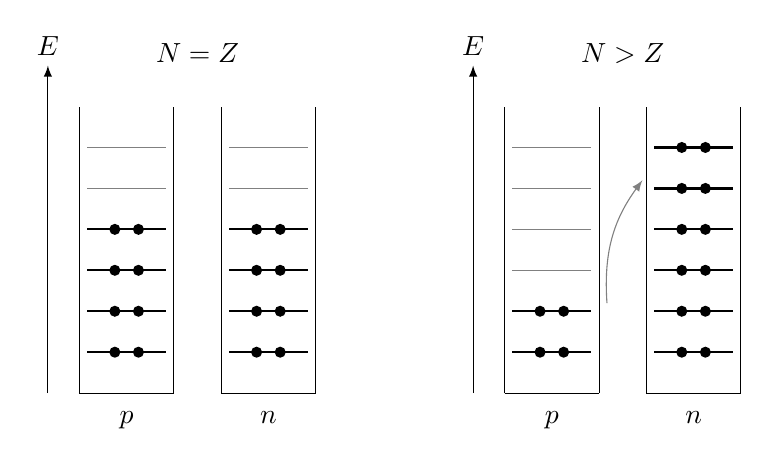
\begin{tikzpicture}[x=1cm, y=0.52cm]
\begin{scope}
  \draw[-latex] (0,0) -- (0,8) node[above] {$E$};
  \node at (1.9,8.3) {$N = Z$};
  \draw (0.4,0) -- (0.4,7) (0.4,0) -- (1.6,0) (1.6,0) -- (1.6,7);
  \node[below] at (1,-0.2) {$p$};
  \draw (2.2,0) -- (2.2,7) (2.2,0) -- (3.4,0) (3.4,0) -- (3.4,7);
  \node[below] at (2.8,-0.2) {$n$};
  \foreach \i in {1,...,4}{
    \draw[thick] (0.5,\i) -- (1.5,\i);
    \draw[thick] (2.3,\i) -- (3.3,\i);
    \fill (0.85,\i) circle (2pt); \fill (1.15,\i) circle (2pt);
    \fill (2.65,\i) circle (2pt); \fill (2.95,\i) circle (2pt);
  }
  \foreach \i in {5,6}{
    \draw[gray] (0.5,\i) -- (1.5,\i);
    \draw[gray] (2.3,\i) -- (3.3,\i);
  }
\end{scope}
\begin{scope}[xshift=5.4cm]
  \draw[-latex] (0,0) -- (0,8) node[above] {$E$};
  \node at (1.9,8.3) {$N > Z$};
  \draw (0.4,0) -- (0.4,7) (0.4,0) -- (1.6,0) (1.6,0) -- (1.6,7);
  \node[below] at (1,-0.2) {$p$};
  \draw (2.2,0) -- (2.2,7) (2.2,0) -- (3.4,0) (3.4,0) -- (3.4,7);
  \node[below] at (2.8,-0.2) {$n$};
  \foreach \i in {1,2}{
    \draw[thick] (0.5,\i) -- (1.5,\i);
    \fill (0.85,\i) circle (2pt); \fill (1.15,\i) circle (2pt);
  }
  \foreach \i in {3,...,6}{ \draw[gray] (0.5,\i) -- (1.5,\i); }
  \foreach \i in {1,...,6}{
    \draw[thick] (2.3,\i) -- (3.3,\i);
    \fill (2.65,\i) circle (2pt); \fill (2.95,\i) circle (2pt);
  }
  \draw[-latex, gray] (1.7,2.2) to[bend left=20] (2.15,5.2);
\end{scope}
\end{tikzpicture}
\caption{Riempimento dei livelli a parità di $A$. A sinistra la configurazione simmetrica, a destra una configurazione asimmetrica, che richiede più energia.}
\label{fig:asimmetria}
\end{figure}

A parità di $A$, la configurazione di minima energia è quella in cui le due scalette sono riempite fino alla stessa altezza, cioè $N = Z$: è la situazione di sinistra in Fig. \ref{fig:asimmetria}. 

Se invece spostiamo $\nu$ nucleoni da una scaletta all'altra, come a destra nella figura, ciascuno di essi deve salire di qualche gradino, perché i livelli bassi dell'altra scaletta sono già occupati. Il primo deve salire di circa $\varepsilon$, il secondo di circa $2\varepsilon$, e così via: il costo complessivo è dell'ordine di
%
\begin{equation}
    \Delta E \sim \nu^2 \varepsilon
\end{equation}
Siccome spostare $\nu$ nucleoni significa passare da $N = Z$ a una differenza $N - Z = 2\nu$, si ha
%
\begin{equation}
    \Delta E \sim \frac{(N-Z)^2}{4} \, \varepsilon
\end{equation}
Resta da capire come dipende $\varepsilon$ da $A$. I nucleoni riempiono un numero di livelli proporzionale ad $A$, ma lo fanno all'interno di una buca la cui profondità non cambia con $A$: lo sappiamo perché $B/A$ è costante, cioè l'energia per estrarre un nucleone è sempre la stessa. Più nucleoni ci sono, quindi, più i livelli si infittiscono nello stesso intervallo di energia
%
\begin{equation}
    \varepsilon \propto \frac{1}{A}
\end{equation}
Mettendo insieme i due risultati, e ricordando che $N - Z = A - 2Z$, si ottiene un contributo negativo all'energia di legame
%
\begin{tcolorbox}[colback=yellow!10!white, colframe=orange!70!black, boxrule=0.8pt]
\begin{equation}
    B_A = - a_A \frac{(A - 2Z)^2}{A}
\end{equation}
\end{tcolorbox}
Questo termine si annulla per $N = Z$ e penalizza qualunque asimmetria, indipendentemente dal verso\footnote{Lo stesso risultato si ottiene in modo più rigoroso trattando il nucleo come un gas di fermioni degenere.}. 

Si noti che è in competizione con il termine coulombiano: il primo favorisce $N = Z$, il secondo spinge ad aggiungere neutroni per diluire la repulsione tra protoni. È dall'equilibrio tra i due che nasce l'eccesso di neutroni dei nuclei pesanti. 

\subsection{Termine di pairing}

C'è un ultimo fatto sperimentale che i termini visti finora non spiegano. Guardando la tabella dei nuclidi stabili si scopre che la grandissima maggioranza ha $Z$ e $N$ \emph{entrambi pari}, mentre i nuclei stabili con $Z$ e $N$ entrambi dispari sono soltanto quattro. Lo stesso effetto si vede nei picchi di ${}^{4}\mathrm{He}$, ${}^{12}\mathrm{C}$ e ${}^{16}\mathrm{O}$ della Fig. \ref{fig:binding_energy}. 

L'origine è ancora quantistica. Due nucleoni dello stesso tipo che occupano lo stesso livello con spin opposto hanno funzioni d'onda spaziali praticamente identiche, quindi si sovrappongono al massimo e l'interazione attrattiva tra loro è la più efficace possibile: una coppia completa è più legata di due nucleoni spaiati su livelli diversi. 

\begin{figure}[htbp]
\centering
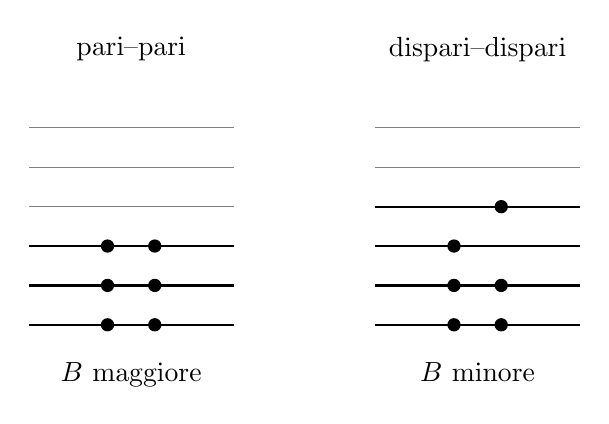
\begin{tikzpicture}[x=1cm, y=0.5cm]
\begin{scope}
  \node at (1.9,8.0) {pari--pari};
  \foreach \i in {1,...,3}{ \draw[thick] (0.6,\i) -- (3.2,\i);
    \fill (1.6,\i) circle (2.4pt); \fill (2.2,\i) circle (2.4pt);}
  \foreach \i in {4,5,6}{ \draw[gray] (0.6,\i) -- (3.2,\i); }
  \node[below] at (1.9,0.3) {$B$ maggiore};
\end{scope}
\begin{scope}[xshift=4.4cm]
  \node at (1.9,8.0) {dispari--dispari};
  \foreach \i in {1,2}{ \draw[thick] (0.6,\i) -- (3.2,\i);
    \fill (1.6,\i) circle (2.4pt); \fill (2.2,\i) circle (2.4pt);}
  \draw[thick] (0.6,3) -- (3.2,3);
  \fill (1.6,3) circle (2.4pt);
  \draw[thick] (0.6,4) -- (3.2,4);
  \fill (2.2,4) circle (2.4pt);
  \foreach \i in {5,6}{ \draw[gray] (0.6,\i) -- (3.2,\i); }
  \node[below] at (1.9,0.3) {$B$ minore};
\end{scope}
\end{tikzpicture}
\caption{Nuclei con tutti i nucleoni appaiati e nuclei con due nucleoni spaiati.}
\label{fig:pairing}
\end{figure}

Si distinguono quindi tre casi:
\begin{itemize}
    \item $Z$ e $N$ pari: tutti i nucleoni sono appaiati e il nucleo guadagna energia di legame;
    \item $Z$ e $N$ dispari: restano un protone e un neutrone spaiati, e il nucleo ne perde;
    \item $A$ dispari: resta un solo nucleone spaiato, caso intermedio che si assume come riferimento.
\end{itemize}
Il termine corrispondente è quindi
%
\begin{tcolorbox}[colback=yellow!10!white, colframe=orange!70!black, boxrule=0.8pt]
\begin{equation}
    \delta_p =
    \begin{cases}
        + \dfrac{a_p}{\sqrt{A}} & Z, N \text{ pari} \\[8pt]
        - \dfrac{a_p}{\sqrt{A}} & Z, N \text{ dispari} \\[8pt]
        0 & A \text{ dispari}
    \end{cases}
\end{equation}
\end{tcolorbox}
dove la dipendenza da $A$ è ricavata empiricamente dai dati e tiene conto del fatto che l'effetto si diluisce al crescere del numero di nucleoni. 

Questo termine spiega in particolare la forte stabilità della particella $\alpha$, che ha $Z = N = 2$.

\subsection{La formula completa}

Mettendo insieme tutti i termini si ottiene la formula semiempirica di massa\mkeyword{formula semiempirica di massa}
%
\begin{tcolorbox}[colback=yellow!10!white, colframe=orange!70!black, boxrule=0.8pt]
\begin{equation}
    B(A,Z) = a_V A - a_S A^{2/3} - a_C \frac{Z^2}{A^{1/3}} - a_A \frac{(A-2Z)^2}{A} + \delta_p
    \label{eq:semf}
\end{equation}
\end{tcolorbox}
i cui parametri sono ricavati da un fit ai dati sperimentali delle centinaia di specie atomiche di cui è stata misurata la massa con sufficiente precisione

\begin{table}[htbp]
\centering
\begin{tabular}{lc}
\hline
Parametro & Valore [MeV] \\
\hline
$a_V$ & $15,5$ \\
$a_S$ & $16,8$ \\
$a_C$ & $0,72$ \\
$a_A$ & $23$ \\
$a_p$ & $11$ \\
\hline
\end{tabular}
\caption{Parametri della formula semiempirica di massa.}
\label{tab:parametri_semf}
\end{table}

Si noti che il termine coulombiano ha il coefficiente più piccolo di tutti, ma è l'unico a crescere come $Z^2$: è quindi lui a determinare il comportamento dei nuclei pesanti. 

\begin{figure}[htbp]
\centering
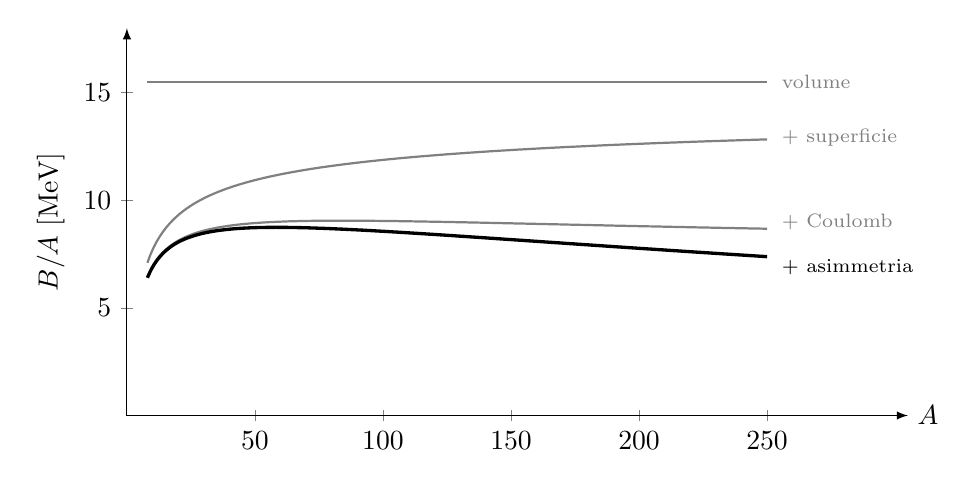
\begin{tikzpicture}
\begin{axis}[
    width=11.5cm, height=6.5cm,
    axis lines=left, axis line style={-latex},
    xlabel={$A$}, ylabel={$B/A$ [MeV]},
    xlabel style={at={(ticklabel* cs:1)}, anchor=west},
    xmin=0, xmax=305, ymin=0, ymax=18,
    xtick={50,100,150,200,250}, ytick={5,10,15},
    clip=false,
]
% --- solo volume
\addplot[gray, thick, domain=8:250, samples=2] {15.5};
\node[anchor=west, font=\scriptsize, gray] at (axis cs:252,15.5) {volume};

% --- volume + superficie
\addplot[gray, thick, domain=8:250, samples=200] {15.5 - 16.8*x^(-1/3)};
\node[anchor=west, font=\scriptsize, gray] at (axis cs:252,12.9) {$+$ superficie};

% --- volume + superficie + Coulomb
\addplot[gray, thick, domain=8:250, samples=300]
 {15.5 - 16.8*x^(-1/3) - 0.72*(x/(2+0.0157*x^(2/3)))^2/x^(4/3)};
\node[anchor=west, font=\scriptsize, gray] at (axis cs:252,9.0) {$+$ Coulomb};

% --- formula completa
\addplot[black, very thick, domain=8:250, samples=300]
 {15.5 - 16.8*x^(-1/3) - 0.72*(x/(2+0.0157*x^(2/3)))^2/x^(4/3)
  - 23*(x-2*x/(2+0.0157*x^(2/3)))^2/x^2};
\node[anchor=west, font=\scriptsize] at (axis cs:252,6.9) {$+$ asimmetria};
\end{axis}
\end{tikzpicture}
\caption{Contributo dei singoli termini della formula semiempirica.}
\label{fig:semf_contributi}
\end{figure}

\section{Parabole di massa}

Inserendo la \eqref{eq:semf} nell'equazione della massa del nucleo si ottiene
%
\begin{equation}
    M(Z,A) = Z m_p + (A - Z) m_n - B(A,Z)
\end{equation}
Fissando $A$ si ottiene la massa a parità di numero di nucleoni, e la dipendenza da $Z$ risulta \emph{quadratica}
%
\begin{tcolorbox}[colback=yellow!10!white, colframe=orange!70!black, boxrule=0.8pt]
\begin{equation}
    M(Z,A) = a + bZ + cZ^2
\end{equation}
\end{tcolorbox}
Il nucleo più stabile a parità di $A$ è quello che minimizza la massa, cioè quello che massimizza l'energia di legame. Imponiamo quindi
%
\begin{equation}
    \frac{\partial B(A,Z)}{\partial Z} = 0 \qquad \Longrightarrow \qquad - \frac{2 a_C Z}{A^{1/3}} + \frac{4 a_A (A - 2Z)}{A} = 0
\end{equation}
da cui
%
\begin{equation}
    \frac{2 a_C Z}{A^{1/3}} + \frac{8 a_A Z}{A} = 4 a_A \qquad \Longrightarrow \qquad Z \left( \frac{a_C A^{2/3}}{A} + \frac{4}{A} \right) = 2 a_A
\end{equation}
e infine
%
\begin{tcolorbox}[colback=yellow!10!white, colframe=orange!70!black, boxrule=0.8pt]
\begin{equation}
    Z_{\min} = \frac{2 a_A A}{4 a_A + a_C A^{2/3}} = \frac{A}{2 + \dfrac{a_C}{2 a_A} A^{2/3}} \simeq \frac{A}{2 + 0,0157 \, A^{2/3}}
    \label{eq:zmin}
\end{equation}
\end{tcolorbox}
Per $A$ piccolo il termine correttivo è trascurabile e si ha $Z \simeq A/2$, cioè lo stesso numero di protoni e neutroni. Per $A$ grande, invece, il termine coulombiano domina: per $A = 239$ si ottiene $Z \simeq 92$, cioè l'uranio. È proprio questo l'andamento che fa incurvare la valle di stabilità verso $N > Z$.\\

Il termine di pairing ha una conseguenza importante su questo quadro. Se $A$ è \emph{dispari} allora $\delta_p = 0$ e le masse si dispongono su un'unica parabola. Se invece $A$ è \emph{pari} il termine di pairing può essere positivo o negativo, e si ottengono \emph{due} parabole traslate del doppio del termine di pairing. 

\begin{figure}[htbp]
\centering
\begin{tikzpicture}
\begin{groupplot}[
    group style={group size=2 by 1, horizontal sep=1.8cm},
    width=6.5cm, height=5cm,
    axis lines=left, axis line style={-latex},
    xlabel={$Z$}, ylabel={$M(Z,A)$},
    xlabel style={at={(ticklabel* cs:1)}, anchor=west},
    ylabel style={at={(ticklabel* cs:1)}, anchor=south west, rotate=-90},
    xtick=\empty, ytick=\empty,
    xmin=42, xmax=58, ymin=0, ymax=10,
    clip=false,
]
\nextgroupplot[title={\small $A$ dispari}]
\addplot[black, thick, domain=42:58, samples=100] {0.14*(x-50)^2+1};
\addplot[only marks, mark=*, mark size=1.2pt, domain=43:57, samples=15] {0.14*(x-50)^2+1};

\nextgroupplot[title={\small $A$ pari}]
\addplot[black, thick, domain=42:58, samples=100] {0.14*(x-50)^2+2.8};
\addplot[black, thick, dashed, domain=42:58, samples=100] {0.14*(x-50)^2+0.6};
\addplot[only marks, mark=*, mark size=1.2pt, domain=44:56, samples=7] {0.14*(x-50)^2+2.8};
\addplot[only marks, mark=*, mark size=1.2pt, domain=43:57, samples=8] {0.14*(x-50)^2+0.6};
\end{groupplot}
\end{tikzpicture}
\caption{Dipendenza della massa da $Z$ a $A$ fissato. Per $A$ pari la parabola tratteggiata corrisponde a $Z$ e $N$ pari, quella continua a $Z$ e $N$ dispari.}
\label{fig:parabole}
\end{figure}

Questo ha un effetto rilevante sui decadimenti: un nucleo può trovarsi sulla parabola superiore e decadere $\beta$ verso quella inferiore, e in alcuni casi il decadimento $\beta$ semplice risulta inibito, lasciando spazio al solo decadimento doppio $\beta$. 

\section{Condizione per il decadimento \texorpdfstring{$\alpha$}{alfa}}

Come applicazione, vediamo per quali nuclei il decadimento $\alpha$ sia energeticamente possibile. Per il processo
%
\begin{equation*}
    {}^{A}_{Z}\mathrm{X} \longrightarrow {}^{A-4}_{Z-2}\mathrm{Y} + {}^{4}_{2}\alpha
\end{equation*}
il $Q$-valore si scrive come
%
\begin{equation}
\begin{aligned}
    Q & = \sum M_{\text{iniz}} - \sum M_{\text{fin}} = M(A,Z) - M(A-4,Z-2) - M(4,2) \\[4pt]
      & = Z m_p + (A-Z) m_n - B(A,Z) - (Z-2) m_p - (A-2-Z) m_n + B(A-4,Z-2) \\
      & \qquad - 2 m_p - 2 m_n + B(4,2) \\[4pt]
      & = B(4,2) + B(A-4, Z-2) - B(A,Z)
\end{aligned}
\end{equation}
Il decadimento è possibile se $Q > 0$, cioè se
%
\begin{tcolorbox}[colback=yellow!10!white, colframe=orange!70!black, boxrule=0.8pt]
\begin{equation}
    B(A,Z) - B(A-4,Z-2) < B(4,2)
\end{equation}
\end{tcolorbox}
Scegliamo adesso una zona della curva in cui la derivata è negativa, cioè $A$ grande, dove possiamo approssimare entrambi i nuclei con la stessa energia di legame media per nucleone $\bar{B}/A$
%
\begin{equation}
    A \frac{\bar{B}}{A} - (A-4) \frac{\bar{B}}{A} < B(4,2) \qquad \Longrightarrow \qquad 4 \frac{\bar{B}}{A} < B(4,2) \simeq 28 \ \mathrm{MeV}
\end{equation}
da cui si conclude che il decadimento $\alpha$ è energeticamente possibile quando
%
\begin{equation}
    \frac{\bar{B}}{A} \lesssim 7 \ \mathrm{MeV}
\end{equation}
condizione verificata soltanto per i nuclei pesanti, dove la curva di Fig. \ref{fig:binding_energy} è ormai scesa sotto questo valore. È questo il motivo per cui gli emettitori $\alpha$ naturali si trovano tutti nella parte alta della tavola periodica.